\subsubsection{Formulario de inicio de sesión}
Para que un cliente pueda iniciar sesión necesita de un formulario donde pueda ingresar sus datos como correo y contraseña.

El formulario que se creó está conformado por dos campos: en el primer campo se le solicita al cliente que ingrese su correo electrónico o su número de teléfono y en el segundo campo se le solicita su contraseña (Ver Figura 6).

    \begin{figure}[H]
        \begin{center}
            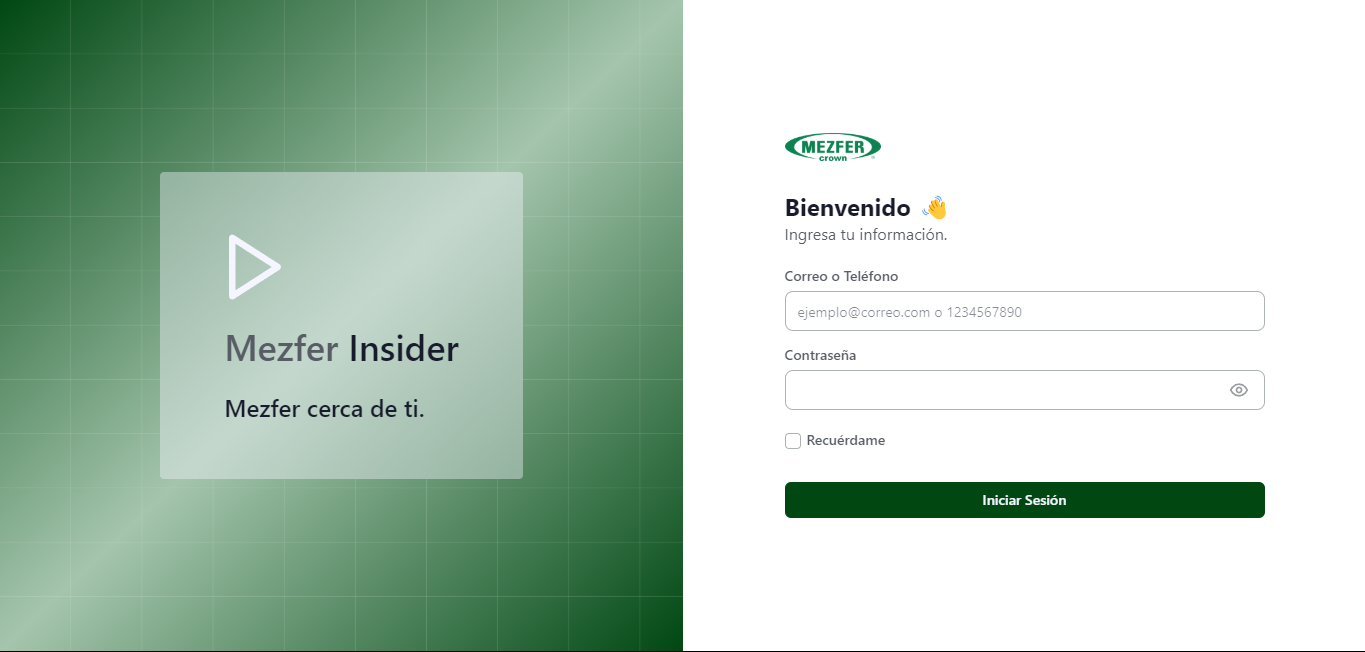
\includegraphics[scale=0.35]{img/actividades/login/Formulario-login.png}
            \caption{Formulario de inicio de sesión de clientes.}
            \label{fig:formulario-login}
        \end{center}
    \end{figure}

El campo de correo electrónico o teléfono está validado mediante expresiones regulares, de esta manera si el cliente escribe algo que no tenga la estructura de alguna de esas dos opciones, no podrá avanzar en el envío de la información. Además, esta validación también permite que el sistema detecte que opción de inicio de sesión se va a usar. Si la validación se cumple para correo electrónico, el objeto que se crea con la información de inicio de sesión del usuario sólo enviará correo y contraseña, y en el Backend se realizará la búsqueda del cliente mediante correo; si la validación se cumple para teléfono, el objeto sólo enviará teléfono y contraseña y se realizará la búsqueda del cliente mediante teléfono.

El cliente no podrá iniciar sesión hasta que ambos campos tengan información y esa información tenga el formato esperado.